\subsection{Blocul de esantionare}

\paragraph{}

Blocul de esantionare este o componenta logica care citeste valorile tensiunii semnalului de intrare la un anumit interval de timp si salveaza in memoria video aceste valori.



\begin{figure}[h]
\centering
\setlength\fboxsep{0pt}
\setlength\fboxrule{0.5pt}
\fbox{
	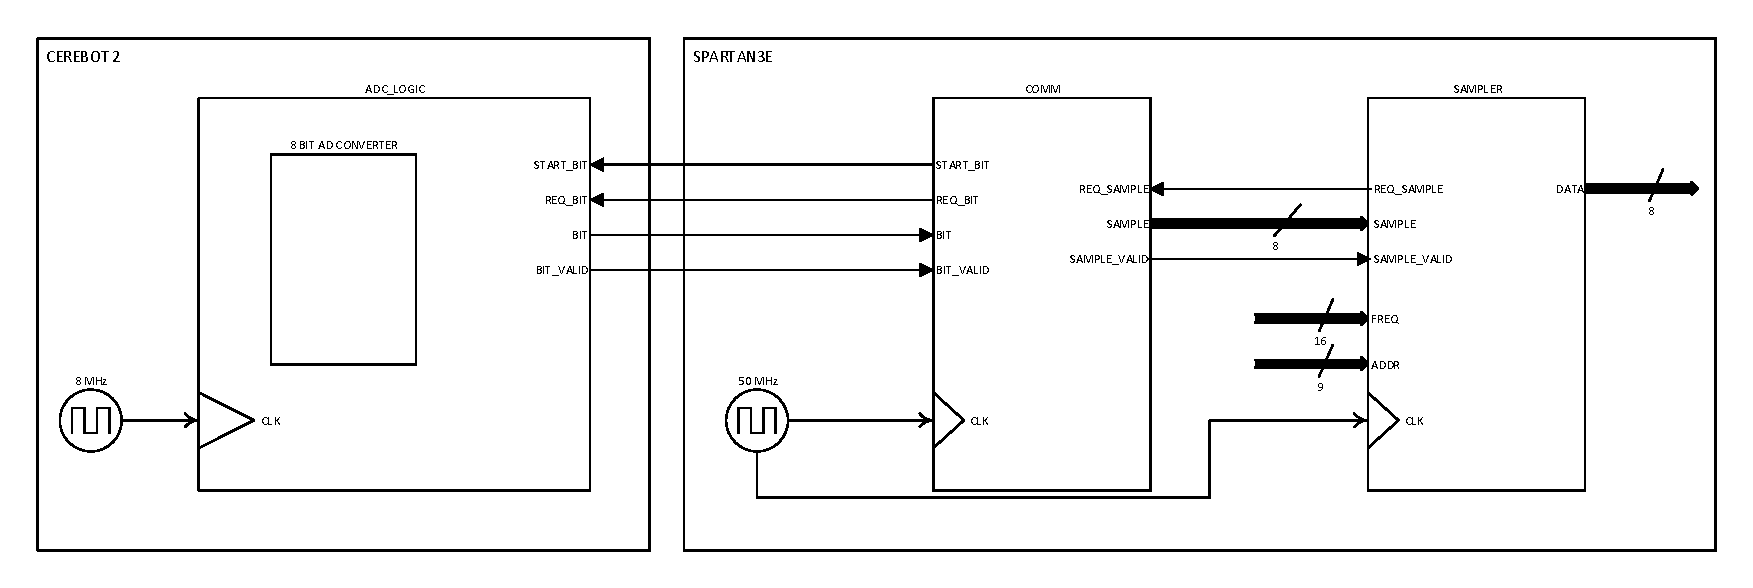
\includegraphics[width=340pt]{oscupdate}
}
\caption{Schema blocului de esantionare cu convertor AD real}
\label{fig:oscupdate}
\end{figure}


\paragraph{}
Acesta este compus din trei subcomponente majore. Componenta ADC, componenta COMM si componenta SAMPLER. Fiecare din aceste componente este un automat de stare.


\paragraph{}
Componenta COMM este responsabila cu transmiterea de informatii dintre convertorul analog digital si componenta de esantionare. Protocolul de comunicare este simplu de inteles si robust. Transmisia bitilor se face in mod serial in pachete de cate 8. In modul IDLE liniile START\_BIT si REQ\_BIT sunt tinute pe zero logic. Cand se doreste transmiterea unui pachet de 8 biti, COMM va trimite un impuls de o lungime fixa (in cazul nostru de 50MHz div 64) pe linia START\_BIT. Dupa o anumita perioada COMM va incepe sa trimita impulsuri pe linia REQ\_BIT de aceiasi lungime cu impulsul de pe START\_BIT. Placuta CEREBOT va detecta aceste impulsuri ca intreruperi externe. Dupa ce s-a trimis un impuls pe REQ\_BIT, COMM va intra intr-o stare de asteptare pana cand linia BIT\_VALID va deveni 1 logic. Este obligatoriu ca aceasta linie sa fie tinuta pe 1 logic pana cand se va transmite un alt impuls pe REQ\_BIT. COMM va citi bitul de pe linia BIT intr-un registru de deplasare, iar mai apoi va trimite din nou o cerere REQ\_BIT pana cand registrul de deplasare este plin.


\begin{figure}[h]
\centering
\setlength\fboxsep{0pt}
\setlength\fboxrule{0.5pt}
\fbox{
	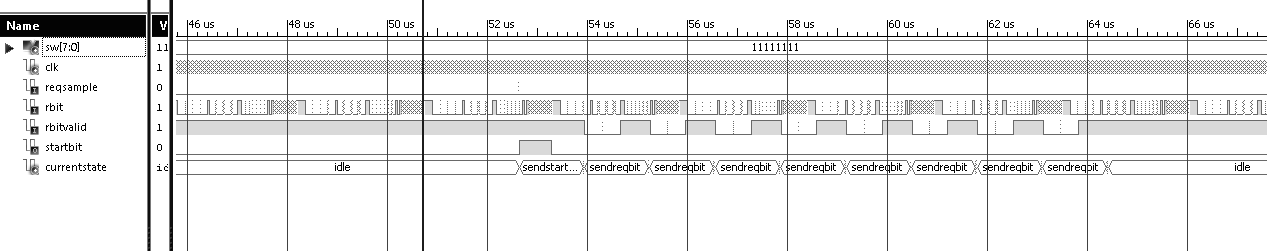
\includegraphics[width=340pt]{waveform-COMM}
}
\caption{Formele de unda pentru COMM}
\label{fig:waveform-COMM}
\end{figure}
\clearpage

\paragraph{}
COMM este un automat de stare. In continuare este prezentata o schema cu tranzitiile intre stari. Starile auxiliare BEGIN* exista deoarece in ele se va intializa un numarator care va avea rolul de a genera impulsuri de o lungime mai mare decat durata tactului de pe placuta FPGA. Avem nevoie de impulsuri mai lungi deoarece placuta CEREBOT2 nu poate detecta intreruperi care sunt mai scurte decat durata clock-ului propriu (8 MHz).

\begin{figure}[h]
\centering
\setlength\fboxsep{0pt}
\setlength\fboxrule{0.5pt}
\fbox{
	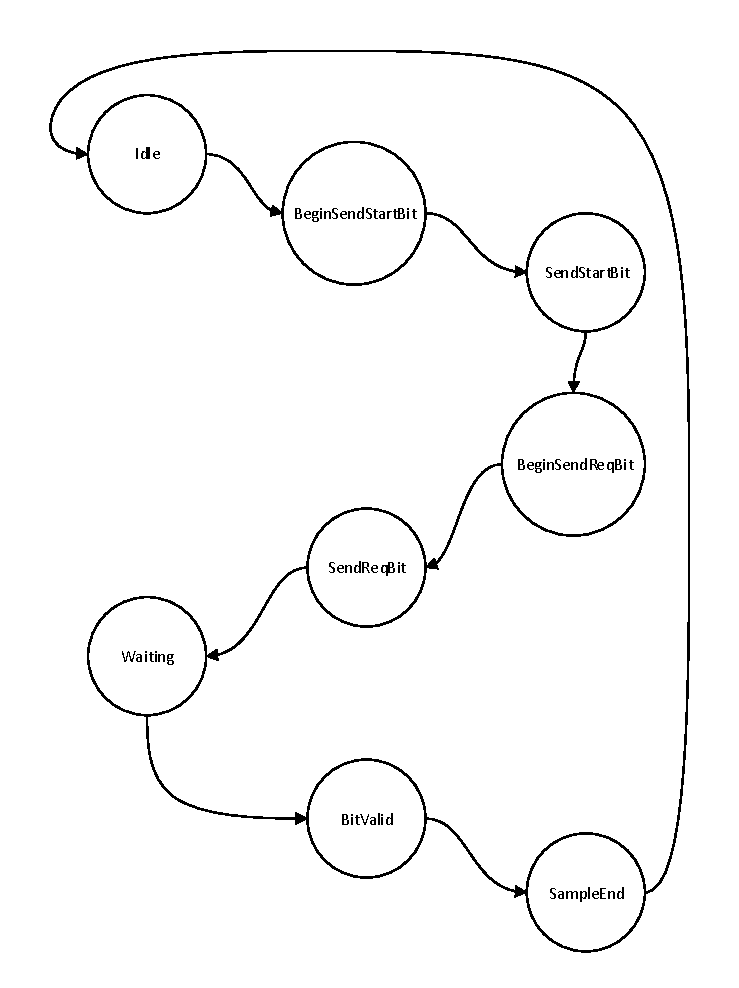
\includegraphics[width=300pt]{COMM-automata}
}
\caption{Diagrama cu tranzitii de stare}
\label{fig:COMM-automata}
\end{figure}
\clearpage


\paragraph{}
Componenta SAMPLER are rolul de declansa conversia analog digitala cu ajutorul bitului REQ\_SAMPLE si a salva valoarea din magistrala SAMPLE cand bitul SAMPLE\_VALID devine 1 intr-o locatie din memoria interna. Memoria video are dimensiunea de 512 x 8 si in ea se vor regasi toate esantioanele capturate. 

\paragraph{}
Frecventa de esantionare este controlata cu variabila FREQ. Aceasta este conectata la SWITCH-urile placutei FPGA si reprezinta numarul de CLK-uri de durata 20ns pe care unitatea sa le astepte intre doua esantioane consecutive.
\(\nu = \frac{1}{ConversionTime + 20ns * FREQ}\)


\paragraph{}
In interiorul componentei se foloseste un registru in care se afla valoarea curenta a adresei de scriere a memoriei. Dupa fiecare esantion capturat valoarea din registru se incrementeaza cu 1, astfel urmatorul sample va fi salvat in continuare in memorie. Exista doua moduri de functionare a osciloscopului: Timp Real si Captura. In modul Timp Real memoria este baleiata si actualizata in mod continuu, in timp ce in modul Captura memoria este actualizata doar atunci cand se detecteaza o schimbare pe portul FREQ.


\paragraph{}
\textbf{Exemplu de functionare}

\begin{figure}[h]
\centering
\setlength\fboxsep{0pt}
\setlength\fboxrule{0.5pt}
\fbox{
	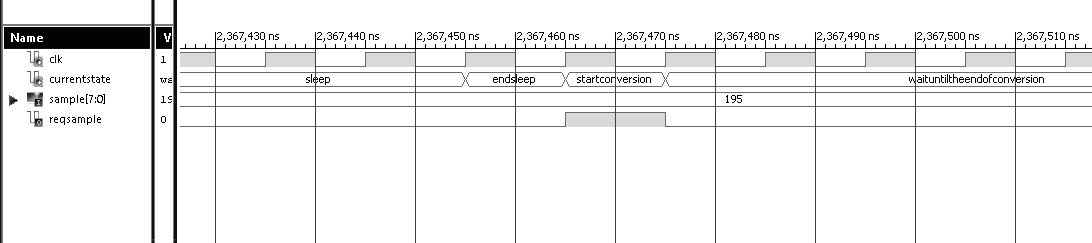
\includegraphics[width=340pt]{waveform-SAMPLER1}
}
\label{fig:waveform-SAMPLER1}
\end{figure}


\begin{figure}[h]
\centering
\setlength\fboxsep{0pt}
\setlength\fboxrule{0.5pt}
\fbox{
	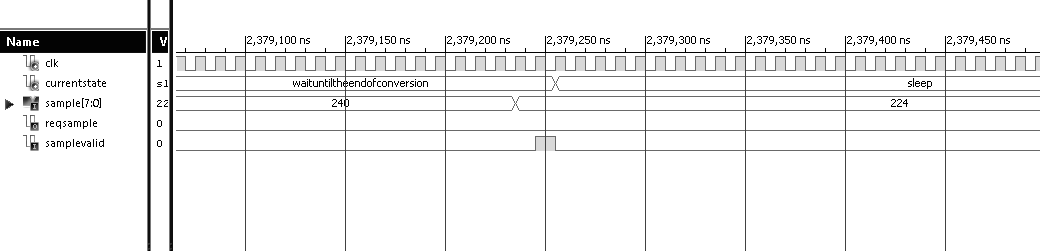
\includegraphics[width=340pt]{waveform-SAMPLER2}
}
\label{fig:waveform-SAMPLER2}
\end{figure}

\begin{figure}[h]
\centering
\setlength\fboxsep{0pt}
\setlength\fboxrule{0.5pt}
\fbox{
	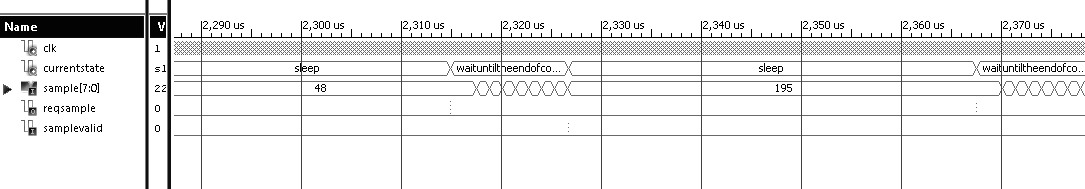
\includegraphics[width=340pt]{waveform-SAMPLER3}
}
\label{fig:waveform-SAMPLER3}
\end{figure}


\clearpage
\begin{figure}[h]
\centering
\setlength\fboxsep{0pt}
\setlength\fboxrule{0.5pt}
\fbox{
	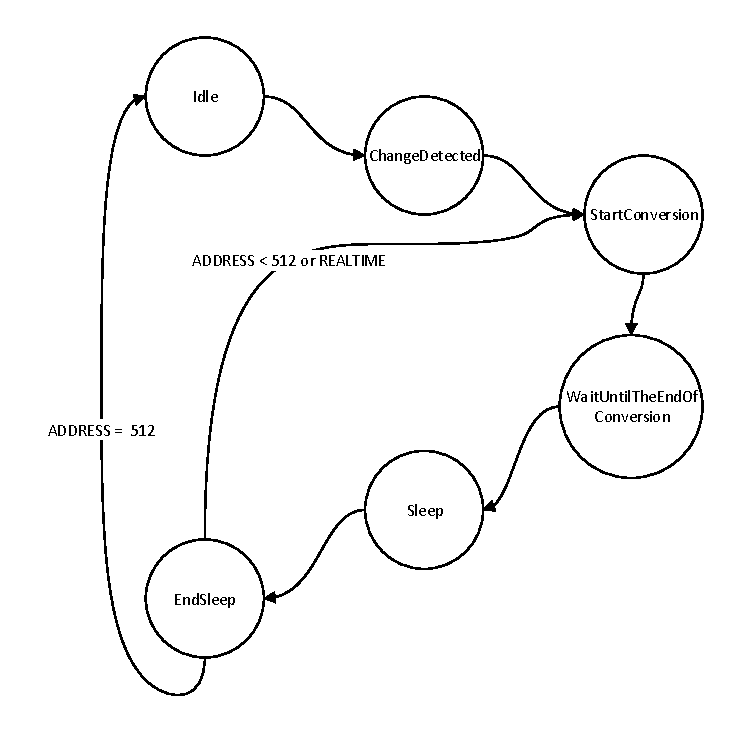
\includegraphics[width=340pt]{SAMPLER-automata}
}
\caption{Diagrama de stare a automatului SAMPLER}
\label{fig:SAMPLER-automata}
\end{figure}



\paragraph{}
Starea \textbf{ChangeDetected} reprezinta starea de initializare a registrului de baleiaj cu adresa 0. Se intra in aceasta stare din \textbf{Idle} cand se detecteaza o schimbare a datelor de pe magistrala \textbf{FREQ}. In starea \textbf{StartConversion} bitul \textbf{REQ\_SAMPLE} devine 1 logic, astfel se semnaleaza o cerere de conversie spre modulul de comunicare (COMM). Se asteapta in starea \textbf{WaitUntilTheEndOfConversion} pana cand bitul \textbf{SAMPLE\_VALID} devine 1 logic iar apoi se intra in starea \textbf{Sleep} in care se incrementeaza un registru la fiecare tact pana la valoarea semnalului \textbf{FREQ}. Cand se atinge aceasta valoare se intra in starea \textbf{EndSleep} de unde se poate continua baleierea adreselor sau inghetarea automatului in starea \textbf{Idle}. Modul de functionare "Timp Real" presupune tranzitia in starea \textbf{StartConversion} iar modul "Captura" tranzitia in starea \textbf{Idle}.


\clearpage

\paragraph{}
Protocolul de comunicare este implementat pe placuta CEREBOT2 folosind intreruperile externe. Cand se detecteaza o tranzitie de tip front crescator al bitului START\_BIT se va genera o intrerupere in care se cere o conversie AD. Valoarea unui registru (de stare) va fi setata pe Waiting. Cand conversia AD este terminata se va genera o alta intrerupere unde se salveaza valoarea convertita intr-un registru. Dupa fiecare intrerupere REQ\_BIT  se va trimite spre iesire valoarea convertita, se va face 1 logic BIT\_VALID iar apoi  registrul se deplasa cu un bit. Daca conversia nu este gata cand vine prima cerere REQ\_BIT vom astepta pana cand va fi gata intr-o stare de Wait (while(1)). BIT\_VALID va deveni 0 de fiecare data cand se executa bucla principala a programului.




\paragraph{}
Pentru testarea in simulator noi am folosit un bloc care genereaza esantioane pseudo- aleatoare cu bistabile si porti xor. Aceasta componenta respecta interfata de comunicare COMM si este o masina de stare.


\begin{figure}[h]
\centering
\setlength\fboxsep{0pt}
\setlength\fboxrule{0.5pt}
\fbox{
	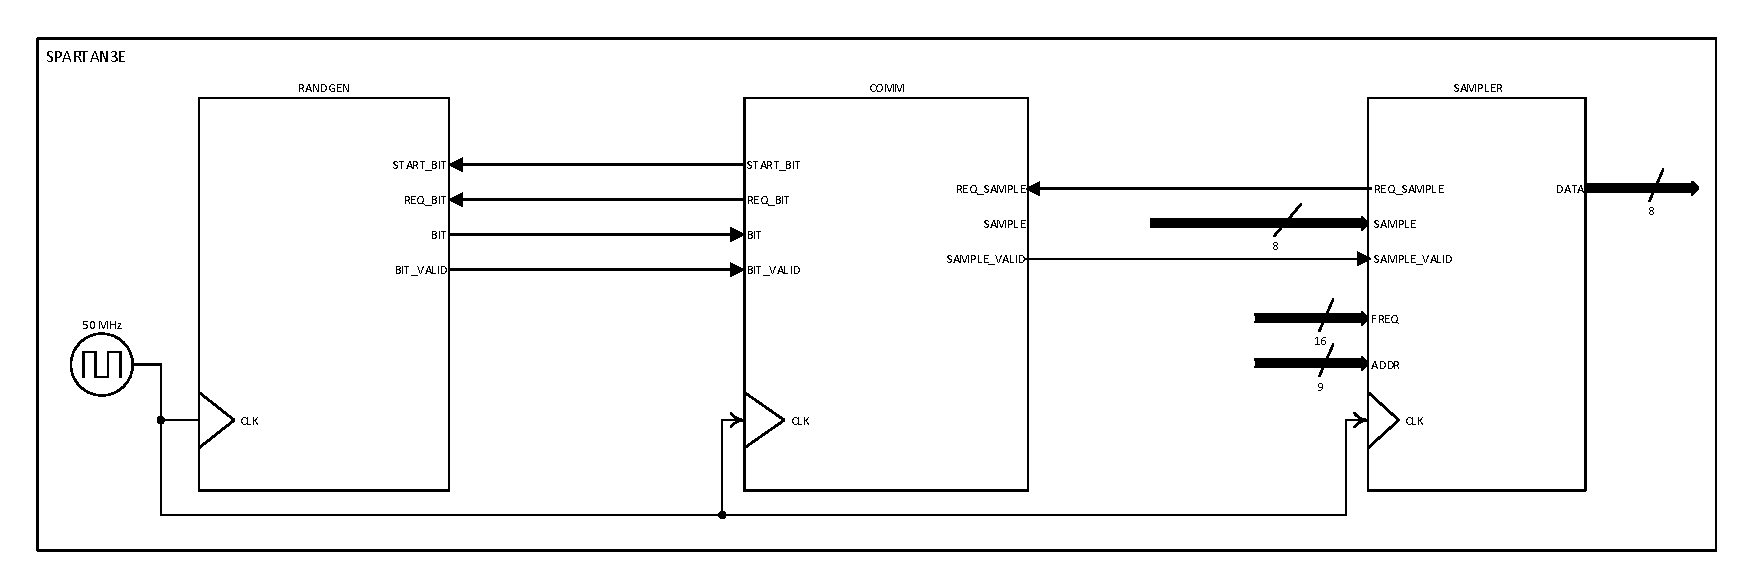
\includegraphics[width=340pt]{oscupdate-rand}
}
\caption{Schema blocului de esantionare cu generator de valori aleatoare pentru testarea in simulator}
\label{fig:oscupdate-rand}
\end{figure}